\chapter{Concepts}
\label{ch:concepts}

\section{Background Information for CNN and GCN}
\txtb{Sentence Bag:}
Sentence Bag(SB) is similar to Bag-of-Words(BoW) representation, with preserving the order of word occurrences. Many Deep Learning algorithms use BoW, but the word order is never stored, as a result, prediction of next word occurrence is hindered. This model generated a data set DS represented as $D = \{S_{(x_i,y_i)}|,i = 1,2,...\}$ and a sentence bag $S_{(x_i,y_i)}$ is a set of sentences with both entities $x_i$ and $y_i$. Yet, it does not store the relation of $x_i$ and $y_i$, and only the order in which entities occurred in a sentence.

\newpar
\txtb{Knowledge Graph:}
Knowledge Graph (KG) consists of triples <$x_i, r_i, y_i$> where $r_i$ is the relationship of entities $x_i$ and $y_i$. This form of representation for KG represents a way to learn about vector embedding of both entities along with relation in a low-dimensional space. 

\newpar
\txtb{Entity Type:}
An entity type $T_{e_i}$ for any entity $e$, helps distinguish $e$ from other entities. Fine-grained entity types suggested by Mintz et al.\cite{mintz2009distant} increase the chances for prediction of relation between two entities.  For example, as shown in Fig.\cite{bibid}, \txti{"How to Start a Company"} is \txti{"book"}. With the $T_{e_i}$ knowledge, prediction of relation between \txti{Jane Doe} and \txti{"How to Start a Company"} from \txti{FounderOf} and \txti{AuthorOf}.

\newpar
\txtb{Relation Path:}
Relation path $p$ in DSRE is defined as a path between a set of entities ($p = {x, e_1,...e_{ln}, y}$) whose relationship flows between entities $x$ and $y$ via $ln$ entities. More the number of entities, larger the path. This is of a concern, when used in a Deep Neural Networks, which will be discussed later. Path $p$ is shown in the figure\cite{bibid}

%\ce{$x$->$[\ce{S_{(x,e_1)}}]$${\ce{e_1}}$->$[\ce{S_{(e_1,e_2)}}]$${\ce{[Hg^{II}I4]^2-}}$ }

%\ce{$x$ ->[\ce{S_{(x,e_1)}}] {\ce{$e_1$}} -> [\ce{S_{(e_1,e_2)}}] {\ce{$e_2$}}} %%%%%%%add image%%%%%%%



\newpage
\section{Encoder}
An encoder is a network (CNN, FC, RNN, etc.) that takes the input, and gives a feature map/vector/tensor as output. The feature vector contains the information and features, that represents the input. An encoder is often coupled with a decoder that takes feature vector as input and tries to produce output that is closest to the original input before encoding.

\newpar
Encoder as a common usage pattern of RNN is utilized to explain encoder in brief. Specifically, an unrolled RNN is considered apt for the use-case.


%\begin{figure}[h!]
	%\centering
	%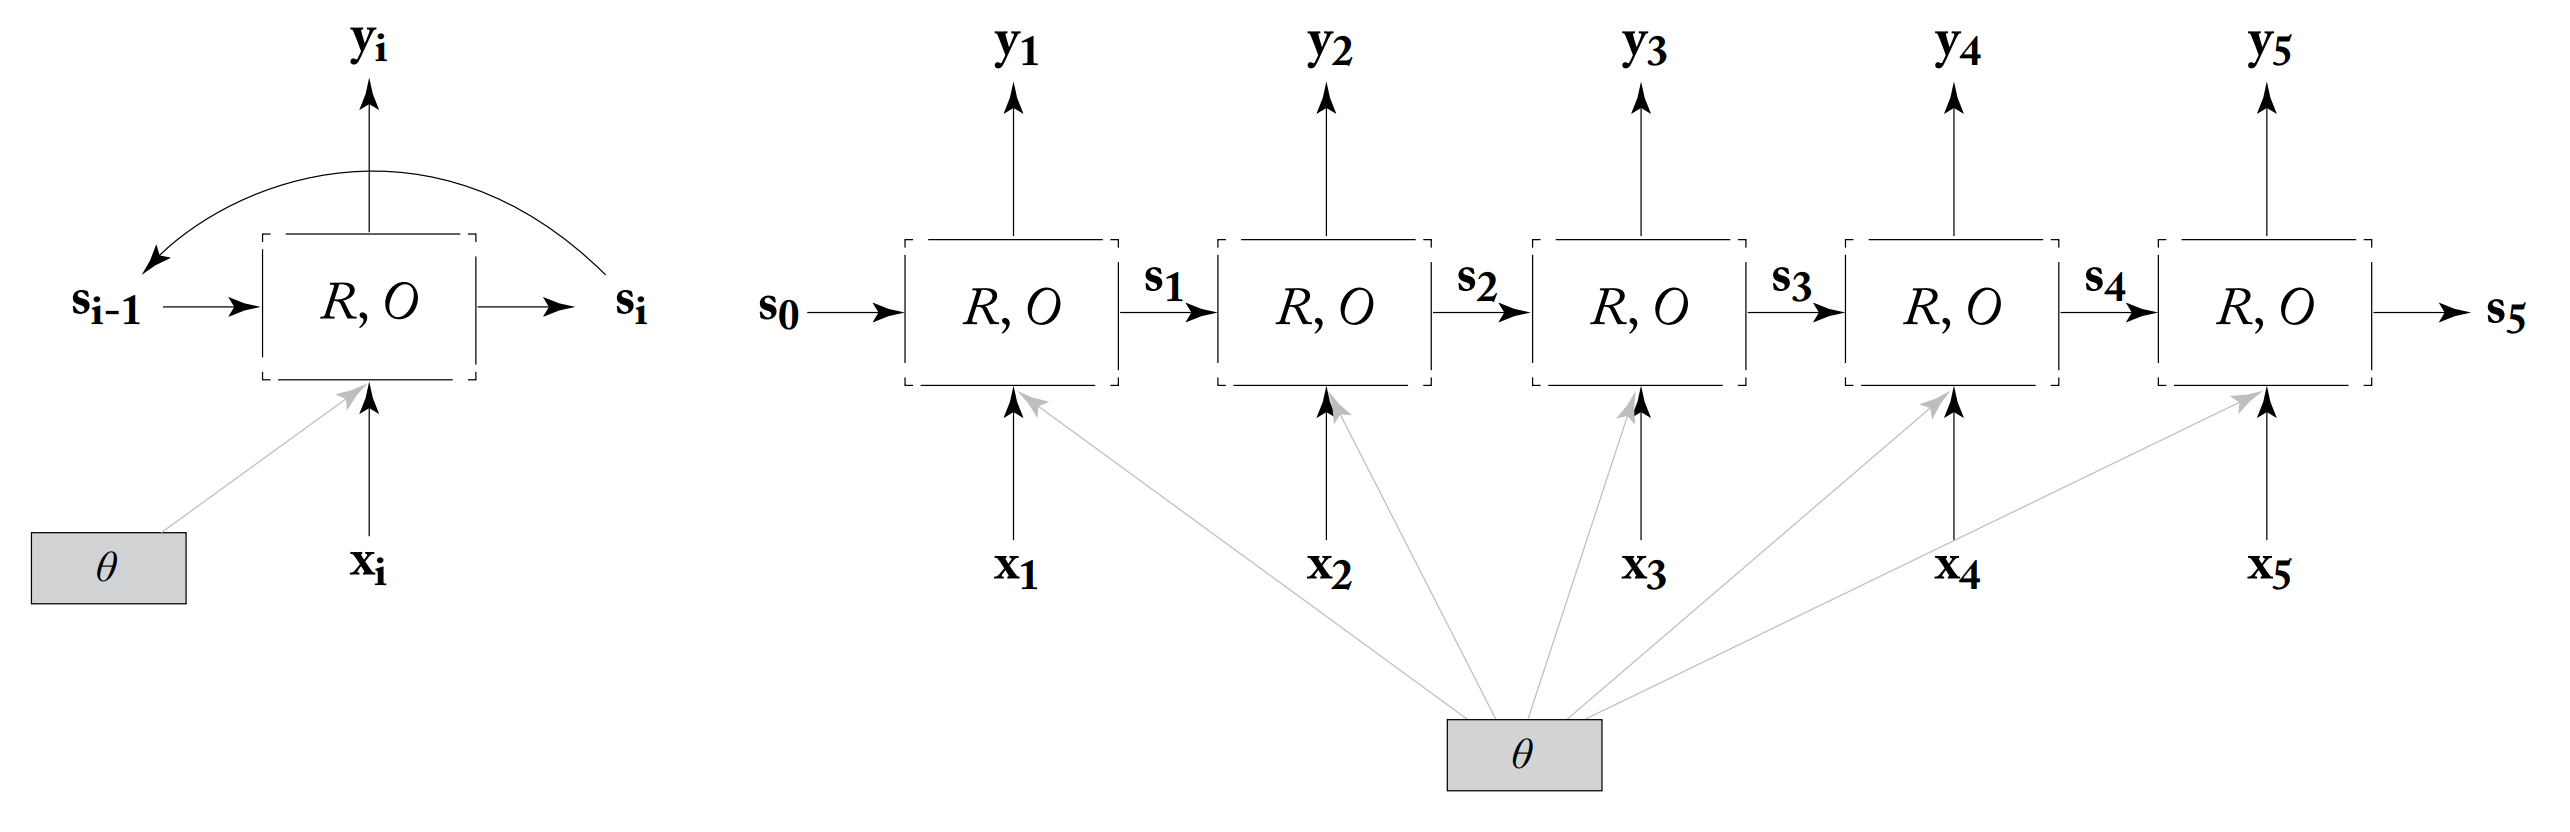
\includegraphics[scale=0.15]{figures/RNN.PNG}
	%\caption{RNN Example}
	%\label{fig:rnn1}
%\end{figure}

\begin{figure}[h!]
	\centering
	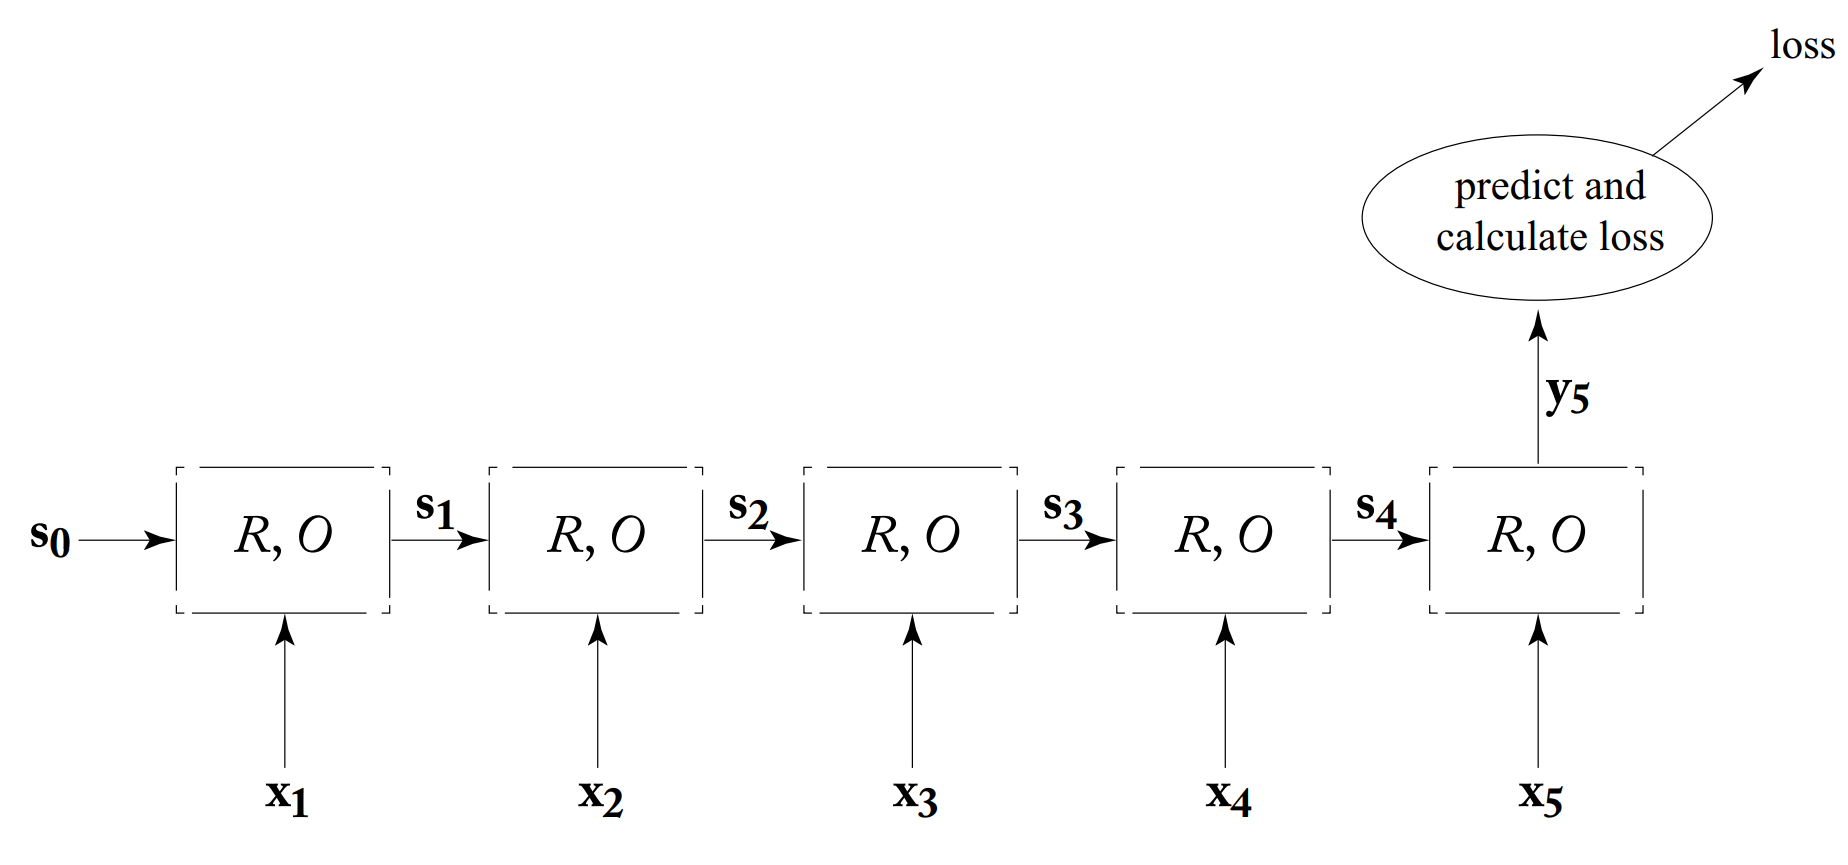
\includegraphics[scale=0.15]{figures/RNNencoder.PNG}
	\caption{RNN Encoder}
	\label{fig:rnn2}
\end{figure}



\section{LSTM Cell: Long-Short-term Memory Cell}

Long Short Term Memory networks(LSTMs)\cite{hochreiter1997long} are a type of RNN, enable to learn long-term dependencies. A simple LSTM cell consists of four gates, namely, Forget gate $f_t$, Input gate $i_t$, Gate gate $\widetilde{C_t}$ and Output gate $o_t$. $h_{(t-1)}$ is the output from previous state, $x_t$ is the input, $h_t$ is the output of present state, $\sigma$ represents a sigmoid function, $C_t$ and $C_{t-1}$ represent cell state. Equations \cref{eq1} represent the gate operations where $b$ and $W$ are model parameters.

\begin{figure}[h!]
	\centering
	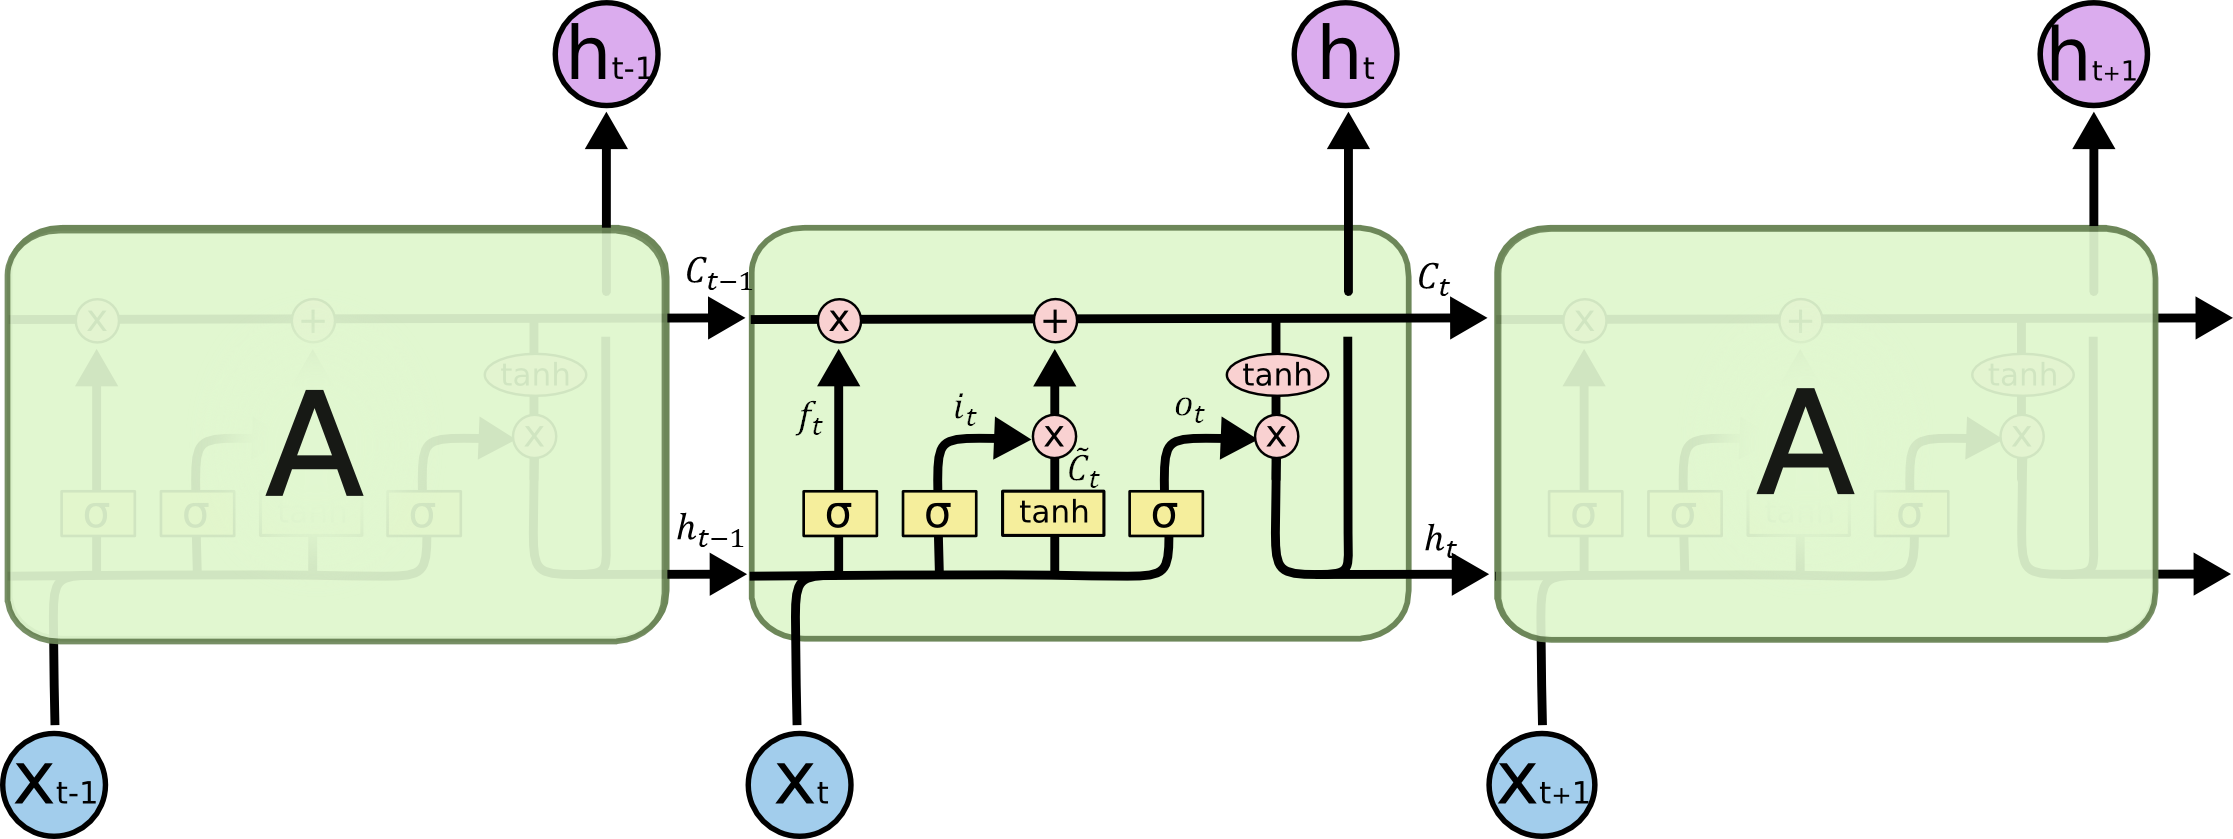
\includegraphics[scale=0.40]{figures/LSTMARCH.PNG}
	\caption{Simplified LSTM Example \cite{colah}}
	\label{fig:lstmsim}
\end{figure}

\begin{subequations}
	\label{eq1}
	\begin{align}
		\displaystyle f_t =\sigma \left(W_f \cdot\left[h_{t-1},x_t\right] + b_f\right) \label{equ:one} \\
		\displaystyle i_t =\sigma \left(W_i \cdot\left[h_{t-1},x_t\right] + b_i\right) \label{equ:two} \\
		\displaystyle \widetilde{C_t} = \tanh \left(W_C \cdot \left[h_{t-1},x_t\right] + b_C\right) \label{equ:three} \\
		\displaystyle C_t = f_t * C_{t-1} + i_t * \widetilde{C_t} \label{equ:four} \\
		\displaystyle o_t =\sigma \left(W_o \cdot\left[h_{t-1},x_t\right] + b_o\right) \label{equ:five} \\
		\displaystyle h_t = o_t * \tanh \left(C_t\right) \label{equ:six}
	\end{align}
\end{subequations}
\newpar





\newpar
LSTMs are embedded into other networks in common to counter vanishing gradients problem and help learning long-term dependencies. This is done by enabling or disabling the gates depending on a model's use-case(target network). A more commonly used variant of LSTMs is Gate Recurrent Unit (GRU). Greff et al.,\cite{greff2016lstm} discuss LSTMs in detail about the popular variants.

\section{GCN : Graph Convolution Network}

The extention of deep neural networks to deal with arbitrary graph-structured data are known as Graph Neural Networks (GNNs)\cite{gori2005new,scarselli2008graph}. In recent years, convolutional operations on graph-structured data are generalized into graph convolutional deep neural networks. Graph Convolutional Networks (GCNs) for short\cite{kipf2016semi}. They are categorically divided into two main types, spectral domain and non-spectral domain. Spectral approaches work on the basis of spectral representation of graphs. Kipf et al.\cite{kipf2016semi} proposed a spectral approach based on work done by Joan Bruna et al.\cite{bruna2013spectral} Michäel et al.\cite{defferrard2016convolutional}, which designs a GCN with a localized first-order approximation of spectral graph convolutions. Non-spectral approaches, perform  convolutions directly on the graph.

\newpar
Commonly, GCNs have two or more hidden layers, where information in the graph is embedded into as eigen vectors by learning some non-linear function. Convolution is the process of applying some filter on the graph data so as to reduce the size of feature matrix into a smaller vector representation. Feature matrix(adjacency matrix) of a graph as shown in Fig. has many empty cells. It is easier to compute on small graphs, but memory overhead increases as real world data-sets are very large. Matrix multiplication with an identity matrix, will reduce the size of adjacency matrix to a vector meanwhile preserving the data. In a GCN, Input will be the first layer and output will be the last layer, in between, there can be many hidden convolution layers with individual non-linear functions. A very simple form of layer-wise propagation rule would be of the form\cite{kipf2016semi},  where $f$ is approximation , $\sigma\left(\cdot\right)$ is a non linear activation function, $H^{\left(l\right)}$ is the graph-level output and $W^{\left(l\right)}$ is the weight matrix for $l$-th neural network layer. $L$ is the number of layers and $l \in L$. $H^{\left(0\right)} = X$ is the input $H^{\left(L\right)} = Z$ is the output

\begin{subequations}
	\label{eq2}
	\begin{align}
	\displaystyle f\left(H^{\left(l\right)},A\right) =\sigma \left(AH^{\left(l\right)}W^{\left(l\right)}\right)
	\end{align}
\end{subequations}
\begin{figure}[h!]
	\centering
	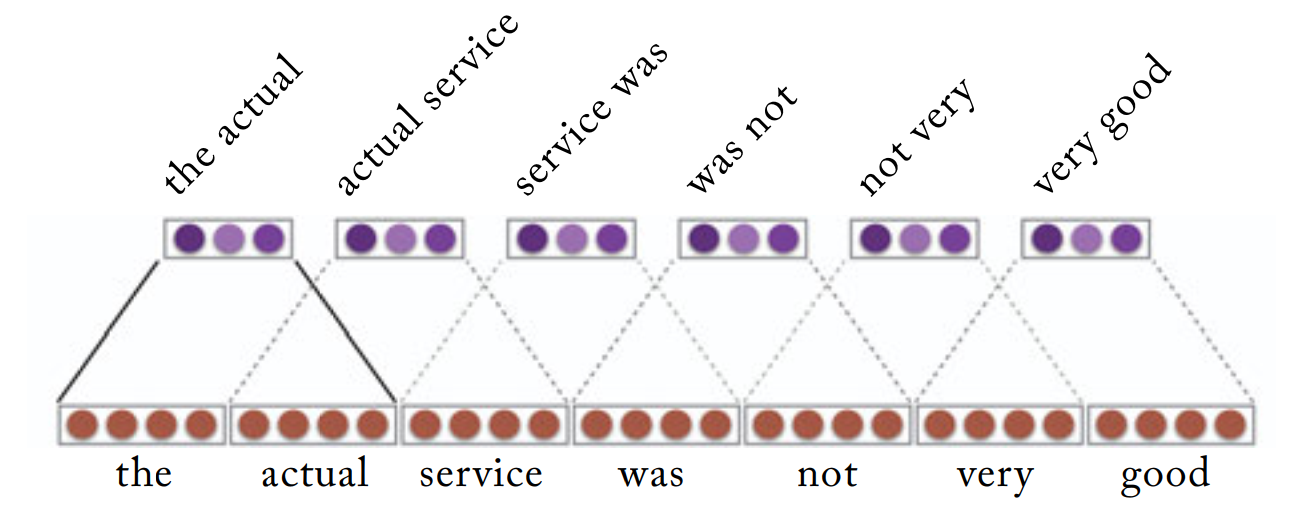
\includegraphics[scale=0.15]{figures/convolution.PNG}
	\caption{convolution Example}
	\label{fig:con}
\end{figure}

